

\documentclass[DIV=calc, paper=a4, fontsize=10pt]{scrartcl}
\usepackage{makeidx}
\usepackage{graphicx}
\usepackage{flushend}
\usepackage{amssymb}


\usepackage{lmodern}
\usepackage[left=1.5cm,right=1.5cm,top=1.5cm,bottom=2cm]{geometry}
\usepackage{float}		
\bibliographystyle{plain} 
\pagestyle{plain} 
\pagenumbering{arabic}
\usepackage{fancyhdr} 	
\usepackage[T1]{fontenc}
\usepackage[utf8]{inputenc}
\usepackage[spanish]{babel}
\usepackage[spanish,es-tabla]{babel}
\usepackage{hyperref}
\usepackage{graphicx}
\usepackage{siunitx}
\usepackage{lipsum}
\usepackage[protrusion=true,expansion=true]{microtype}
\usepackage{amsmath,amsfonts,amsthm}
\usepackage[svgnames]{xcolor}
\usepackage[svgnames]{xcolor}
\usepackage{booktabs}
\usepackage{fix-cm}
\usepackage{multicol}
\usepackage{url}
\usepackage{cancel}
\usepackage{subfig}
\bibliographystyle{unsrt}

\newenvironment{Figura}
  {\par\medskip\noindent\minipage{\linewidth}}
  {\endminipage\par\medskip}

\usepackage{sectsty}
\allsectionsfont{\usefont{OT1}{phv}{b}{n}}
\usepackage{fancyhdr}
\spanishdecimal{.}
\pagestyle{fancy}
\usepackage{lastpage}
\lhead{}
\chead{}
\rhead{}
\lfoot{}
\cfoot{}
\rfoot{\footnotesize Page \thepage\ of \pageref{LastPage}}
\renewcommand{\headrulewidth}{0.0pt}
\renewcommand{\footrulewidth}{0.4pt}
\usepackage{lettrine}
\newcommand{\initial}[1]{\lettrine[lines=3,lhang=0.3,nindent=0em]{
\color{DarkGoldenrod}{\textsf{#1}}}{}}
\usepackage{titling}
\newcommand{\HorRule}{\color{DarkGoldenrod} \rule{\linewidth}{1pt}}
\pretitle{\vspace{-120pt} \begin{flushleft} \HorRule \fontsize{22}{35} \usefont{OT1}{phv}{b}{n} \color{DarkRed} \selectfont}
\title{Práctica 8. \\ %Aquí va el nombre de la práctica 
Lentes} %Numero de la práctica 
\posttitle{\par
\end{flushleft}
\vskip 0.5em}
\preauthor{\begin{flushleft}\large \lineskip 0.5em \usefont{OT1}{phv}{b}{sl} \color{DarkRed}}
\author{Angel Yair García Pérez \\
Misael Iván Macías Márquez\\
Teodora Irene Ortíz Cruz\\
\small{teodora625@ciencias.unam.mx}\\}
\postauthor{\footnotesize \usefont{OT1}{phv}{m}{sl} \color{Black}
\vspace*{0.1cm} 
Facultad de Ciencias, UNAM
\par\end{flushleft}\HorRule}
\date{20 de Mayo de 2022\\Semestre 2022-2}
\begin{document}
\maketitle
\definecolor{carmine}{rgb}{0.59, 0.0, 0.09}
\begin{abstract}
\textcolor{carmine}{Resumen:} Por medio de distintos métodos experimentales se midieron las distancias objeto-lente, imagen-lente, para algunos casos se midió el tamaño de la imagen. Se hizo un análisis de datos y un análisis gráfico con algunos datos. Con el método objeto infinito se obtuvo que la posición del foco de la lente convergente era ${(10.8\hspace{0.1cm}\pm\hspace{0.1cm}{0.05})\text{ cm}}$ con discrepancia de $16$ y $\Delta_{\%}=0.5\%$, con el método gráfico para la misma lente, se obtuvo un foco posicionado en ${(9.493\hspace{0.1cm}\pm\hspace{0.1cm}{0.087})\text{ cm}}$ con discrepancia de $5$ y $\Delta_{\%}=0.87\%$ y usando el método de Bessel para lentes convergentes se obtuvo que el foco estaba en ${(10.21\hspace{0.1cm}\pm\hspace{0.1cm}{0.03})\text{ cm}}$ con discrepancia de $7$  y $\Delta_{\%}=0.3\%$. Con el método de Bessel para lentes divergentes se obtuvo que el foco de la lente era de ${(-9.53\hspace{0.1cm}\pm\hspace{0.1cm}{0.35})\text{ cm}}$ con una discrepancia de $1.34$ y $\Delta_{\%}=3.5\%$, para la misma lente con el método de desplazamiento imagen se obtuvo que la posición del foco era ${(-9.40\hspace{0.1cm}\pm\hspace{0.1cm}{0.69})\text{ cm}}$ con una discrepancia de $0.86$ y  $\Delta_{\%}=6.9\%$. Con el esferómetro se obtuvo que el foco de la lente convergente era $(9.25\hspace{0.1cm}\pm\hspace{0.1cm}0.03\text{ cm})$ con una discrepancia de $25$ y  $\Delta_{\%}=0.03\%$, el índice de refracción para el lente es $(2 \pm 0.2)$ con una discrepancia de $2.5$y $\Delta_{\%}10\%$. 
\end{abstract}
\section*{\textcolor{carmine}{Introducción.}}
El objetivo de este trabajo es practicar los distintos métodos para encontrar distancias focales de lentes y su índice de refracción para comprobar el modelo teórico propuesto en la literatura\cite{Manual}. La importancia de está practica radica en familiarizarse con los distintos tipos de lentes y con como modifican la imagen. Se espera que se cumpla el modelo teórico propuesto en la literatura \cite{book} y partiendo de los valores de fabrica de los lentes se espera encontrar que el valor del foco de la lente convergente sea de $10 cm$ y el de la divergente sea de $-10cm$ y se espera que la lente convergente tenga un índice de refracción de 1.514.
\subsection*{\textcolor{carmine}{Lentes}} 
A partir de la teoría de refracción en una superficie esférica \cite{Manual} se puede considerar que una lente esta formada por dos superficies esféricas muy cercanas y por medio de un tratamiento algebraico llegar a la ecuación  de la lente delgada \cite{book} De donde se sigue fácilmente que  la ecuación del constructor de lentes y una igualdad más:  
\begin{equation}
    \frac{1}{f}=\frac{(n_{2}-n_{1})}{n_{1}}\left(\frac{1}{R_{1}}-\frac{1}{R_{2}}\right)=\frac{1}{o}+\frac{1}{i}
\end{equation}
Finalmente por medio de un diagrama de rayos como el que se muestra en la Figura 1(a), se puede obtener que la magnificación lateral para lentes delgadas es \cite{book}
\begin{equation}
    M=\frac{h_{i}}{h_{o}}=-\frac{i}{o}
\end{equation}
La capacidad de cada lente para hacer que los rayos de luz converjan o diverjan es denominada potencia óptica de la superficie y la ecuación que la caracteriza es \cite{book}
\begin{equation}
    \frac{1}{f}=(n-1)\left(\frac{1}{R_{1}}-\frac{1}{R_{2}}\right)
\end{equation}
\subsection*{\textcolor{carmine}{Formula de Bessel.}}
Supóngase que se tiene un objeto y una pantalla con una separación fija y en medio de ellos una lente como la que se muestra en la figura 1(b), la cual enfocara una imagen real en solo dos posiciones la separación entre esas dos posiciones también es fija y a partir de escribir las distancias fijas en términos distancia-objeto y distancia-imagen, usando la ec.(3) \cite{article}
\begin{equation}
    f=\frac{b^{2}-a^{2}}{4b}
\end{equation}
Arrojando la condición de que la primer distancia-imagen debe ser positiva y menor que b, es decir $b^{2}-4bf\geq 0$ y por tanto la mayor longitud focal que puede ser medida para una b fija es $f\leq\frac{b}{4}$\cite{article}.\\

\begin{figure}[H]
    \centering
    \subfloat[Diagrama de rayos de una lente delgada \cite{book}]{
    \label{f:Arreglo experimental}
    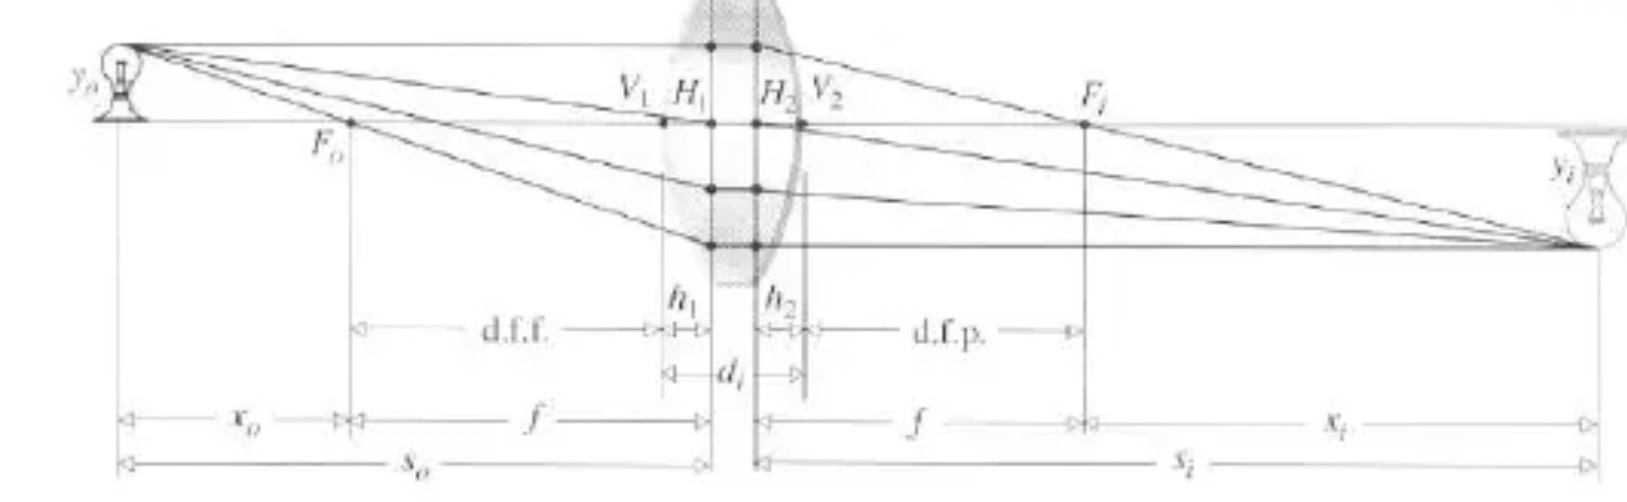
\includegraphics[width=5.5cm]{imagenes/Captura de Pantalla 2022-05-19 a la(s) 13.17.19.png}}
    \subfloat[Diagrama del método de Bessel\cite{article}]{
   \label{f:Lineas}
    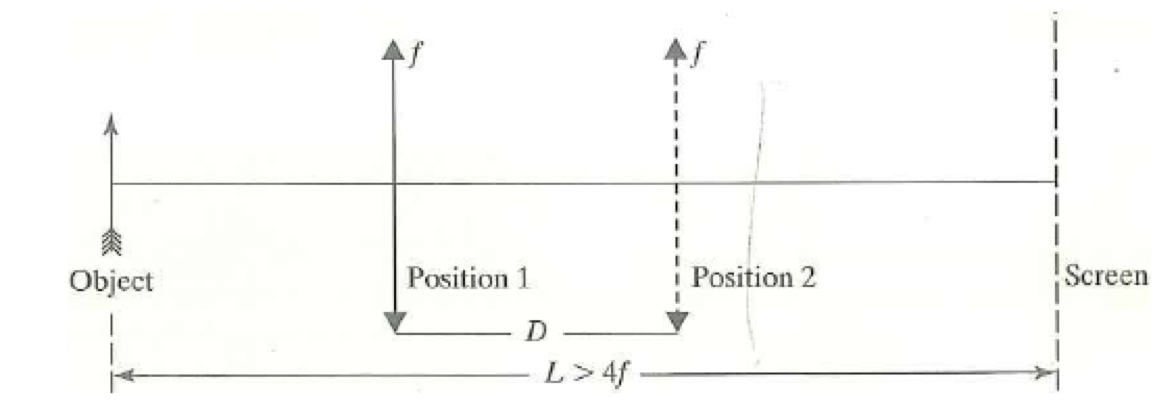
\includegraphics[width=0.35\textwidth]{imagenes/Captura de Pantalla 2022-05-19 a la(s) 13.33.00.png}}
 \caption{Diagramas. En el 1(a) se muestra un diagrama de rayos para una lente donde se puede observar la geometría para obtener las distintas ecuaciones de lentes. En el 1(b) se observa el método de Bessel descrito.}
 \label{f:Desarrollo experimental}
\end{figure}
\section*{\textcolor{carmine}{Desarrollo Experimental}}
\subsection*{\textcolor{carmine}{Objeto Infinito}}
En la mesa del laboratorio se colocó un riel óptico con escala y sobre el se colocó una pantalla y una lente convergente. Para este método se utilizó como objeto lejano un edificio. La pantalla se colocó atrás de la lente y se movió hasta que se proyectara una imagen nítida del edificio como se muestra en la Figura 2(a). Por último se registro la distancia entre la pantalla y la lente con una incertidumbre dada por la escala del riel óptico $\sigma_{ap}=\pm\hspace{0.1cm}0.05\hspace{0.1cm}cm$.
\subsection*{\textcolor{carmine}{Método gráfico.}}
Para este método, sobre el riel se colocó una pantalla y una luz LED plana en forma de flecha como se muestra en la Figura 2(b). El LED se colocó alejado de la lente y se fue acercando cada $5\text{ cm}$ y en cada posición del LED se movió la pantalla hasta que la flecha se viera nítida. Se tomaron las medidas de la distancia objeto-lente y distancia imagen-lente, también se midió la altura del objeto, esta fue de $3.2 cm$ con incertidumbre $\sigma_{ap}=\pm\hspace{0.1cm}0.05\hspace{0.1cm}\text{ cm}$. En las medidas de las distancias se considero una incertidumbre de apreciación, dada por la escala del riel, $\sigma_{ap}=\pm\hspace{0.1cm}0.05\hspace{0.1cm}\text{ cm}$, para algunas distancias se tomó en cuenta una incertidumbre de definición $\sigma_{def}$, ya que para algunas distancias no estaba claro el punto donde la imagen era nítida, para la altura de la imagen se tomó la incertidumbre del vernier $\sigma_{ap}=\hspace{0.1cm}0.005\hspace{0.1cm}\text{ cm}$.
\begin{figure}[H]
    \centering
    \subfloat[\textbf{Arreglo experimental de Objeto Infinito.}Se observa la lente convergente colocada cerca de la pantalla en la cual se forma la imagen de un edificio.]{
    \label{f:Arreglo experimental}
    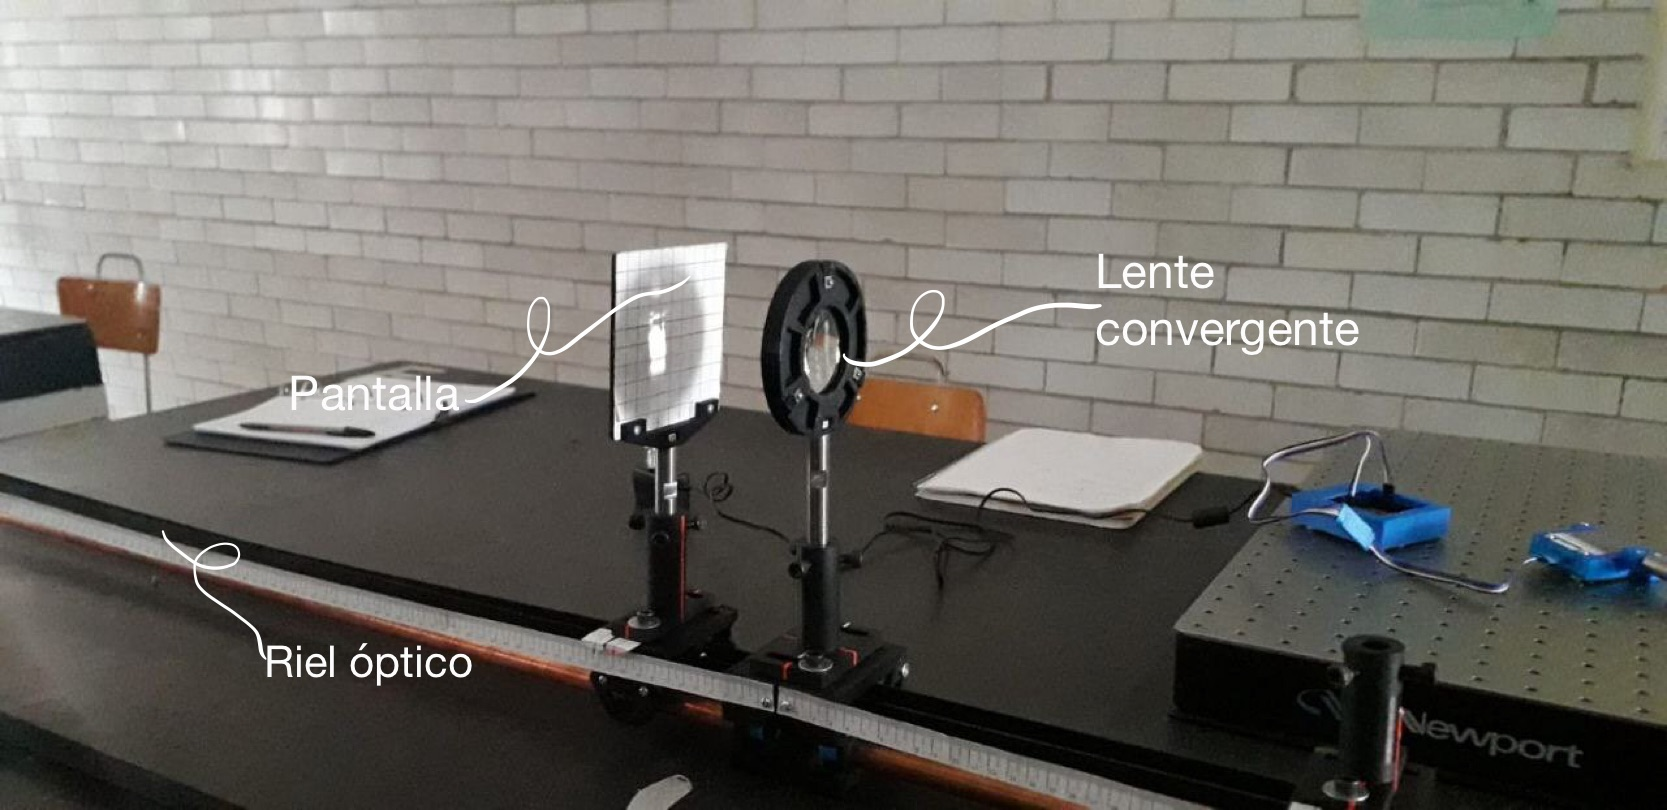
\includegraphics[width=8cm]{imagenes/D6D51F04-1487-4F4E-BD7F-40358443E52F.jpeg}}
    \subfloat[\textbf{Arreglo experimental de Método gráfico.} ]{
   \label{f:Lineas}
    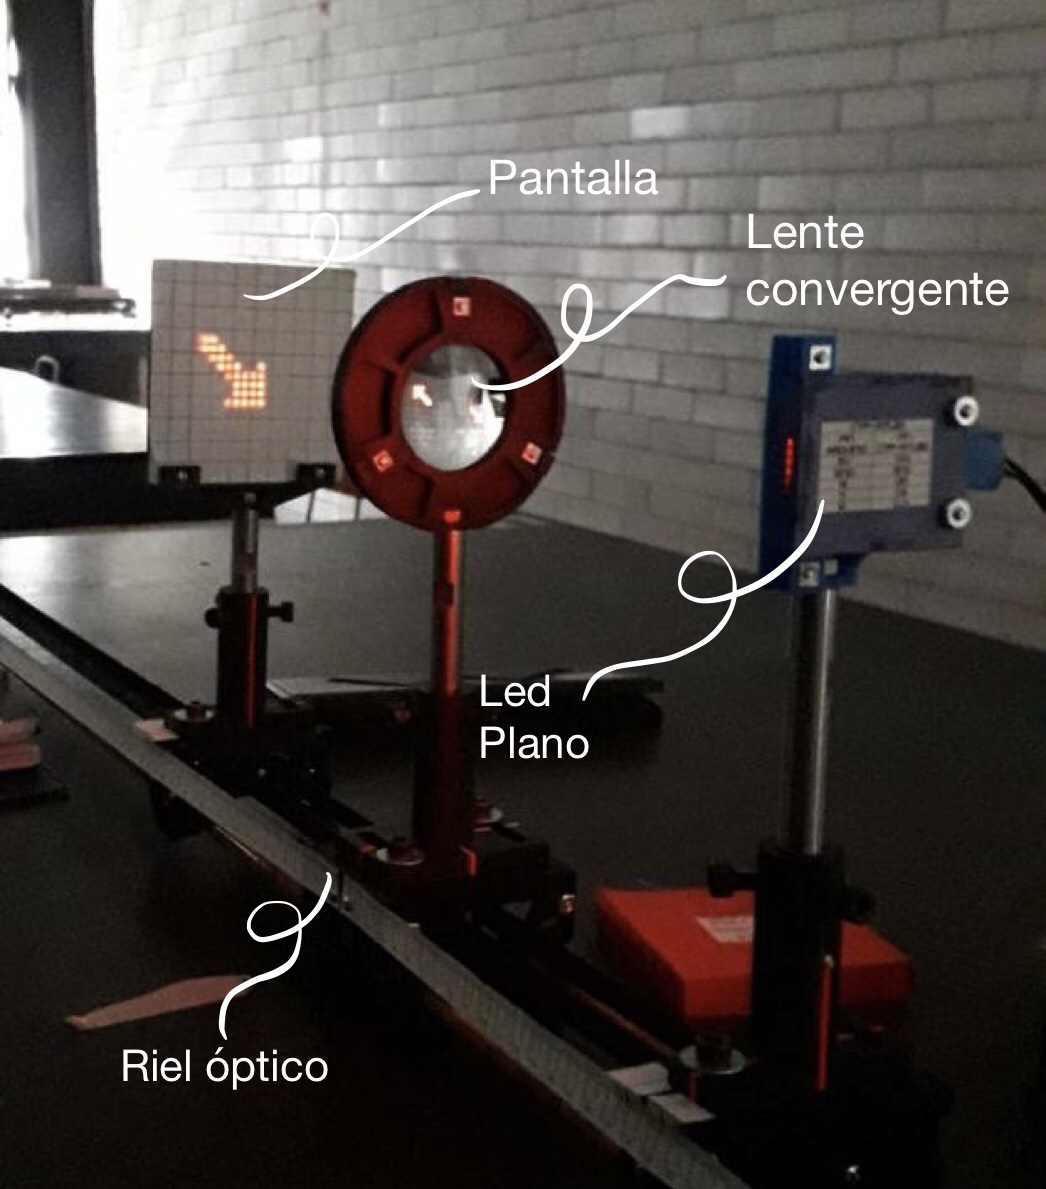
\includegraphics[width=0.19\textwidth]{imagenes/28A802A0-60D7-4890-AE97-B851660139C1.jpeg}}
 \caption{En la figura 2(a) se observa el arreglo experimental utilizado para el método objeto infinito. En la figura 2(b) se observa el arreglo experimental descrito y utilizado en el apartado del método gráfico.}
 \label{f:Desarrollo experimental}
\end{figure}
\subsection*{\textcolor{carmine}{Bessel con una lente covergente.}}
Con el objeto colocado a la orilla de la mesa de trabajo, se colocó la lente convergente y la pantalla sobre el riel óptico con escala. Debido a que la lente estaba fija en el riel se posicionó la pantalla lejana a la lente mientras el objeto se acercó hasta que se observó una imagen nítida como muestra la figura 2(a). Se registraron las distancias con una incertidumbre $\sigma_{ap}=\pm\hspace{0.1cm}0.05\hspace{0.1cm}\text{ cm}$.
Luego se colocó el objeto a la misma distancia a la que estaba antes la pantalla y la pantalla se acercó hasta que llegara a la distancia a la que estaba el objeto. A partir de ello se buscó el punto en el que la imagen proyectada se viera más nítida y fue registrada con la misma incertidumbre. 
\subsection*{\textcolor{carmine}{Bessel para lentes divergentes.}}
Con el objeto colocado a la orilla de la mesa de laboratorio, se colocó la lente divergente y la pantalla sobre la mesa de forma paralela a la cinta métrica. La pantalla se posicionó a más de un metro con una incertidumbre de apreciación $\sigma=\pm\hspace{0.11cm}0.05\hspace{0.11cm}\text{ cm}$.
Luego entre la divergente y la pantalla se colocó la lente convergente como se muestra en la Figura 3(a). Con la lente convergente se cambiaron las posiciones hasta encontrar dos imágenes reales, cada una con un tamaño diferente. Utilizando un vernier se tomaron las medidas de las imágenes producidas por el sistema óptico y se les asoció una incertidumbre  $\sigma_{ap}=\pm\hspace{0.1cm}0.005\hspace{0.1cm}\text{ cm}$.
\begin{figure}[H]
    \centering
    \subfloat[\textbf{Arreglo experimental} Bessel para covergentes.]{
    \label{f:Arreglo experimental}
    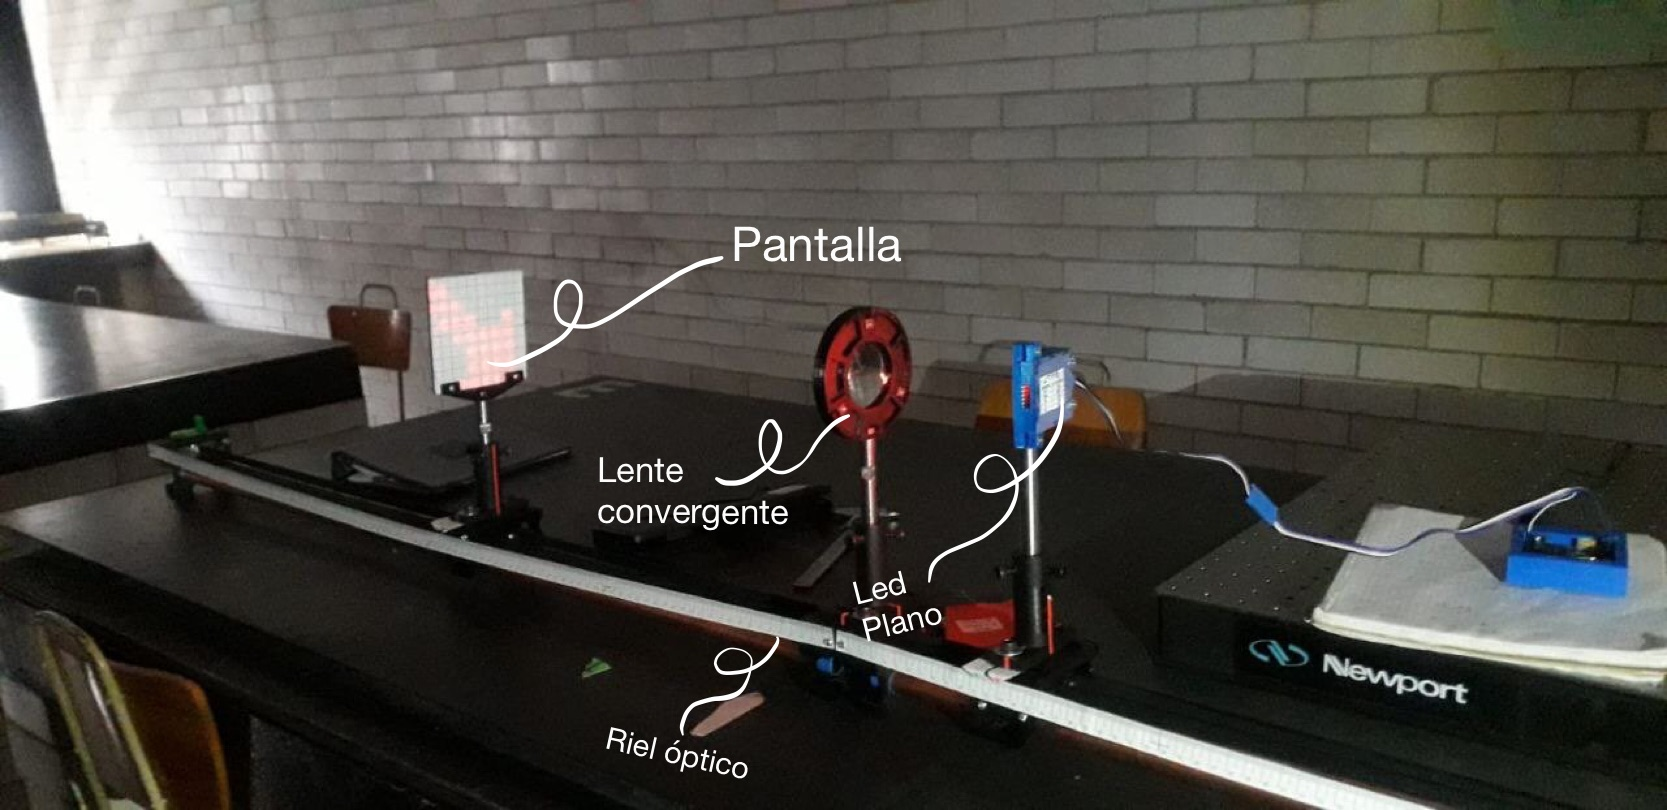
\includegraphics[width=7cm]{imagenes/12DF4E66-9172-4674-B825-CC7990EC0F20.jpeg}}
   \subfloat[\textbf{Arreglo experimental.}Bessel para divergentes ]{
   \label{f:Lineas}
    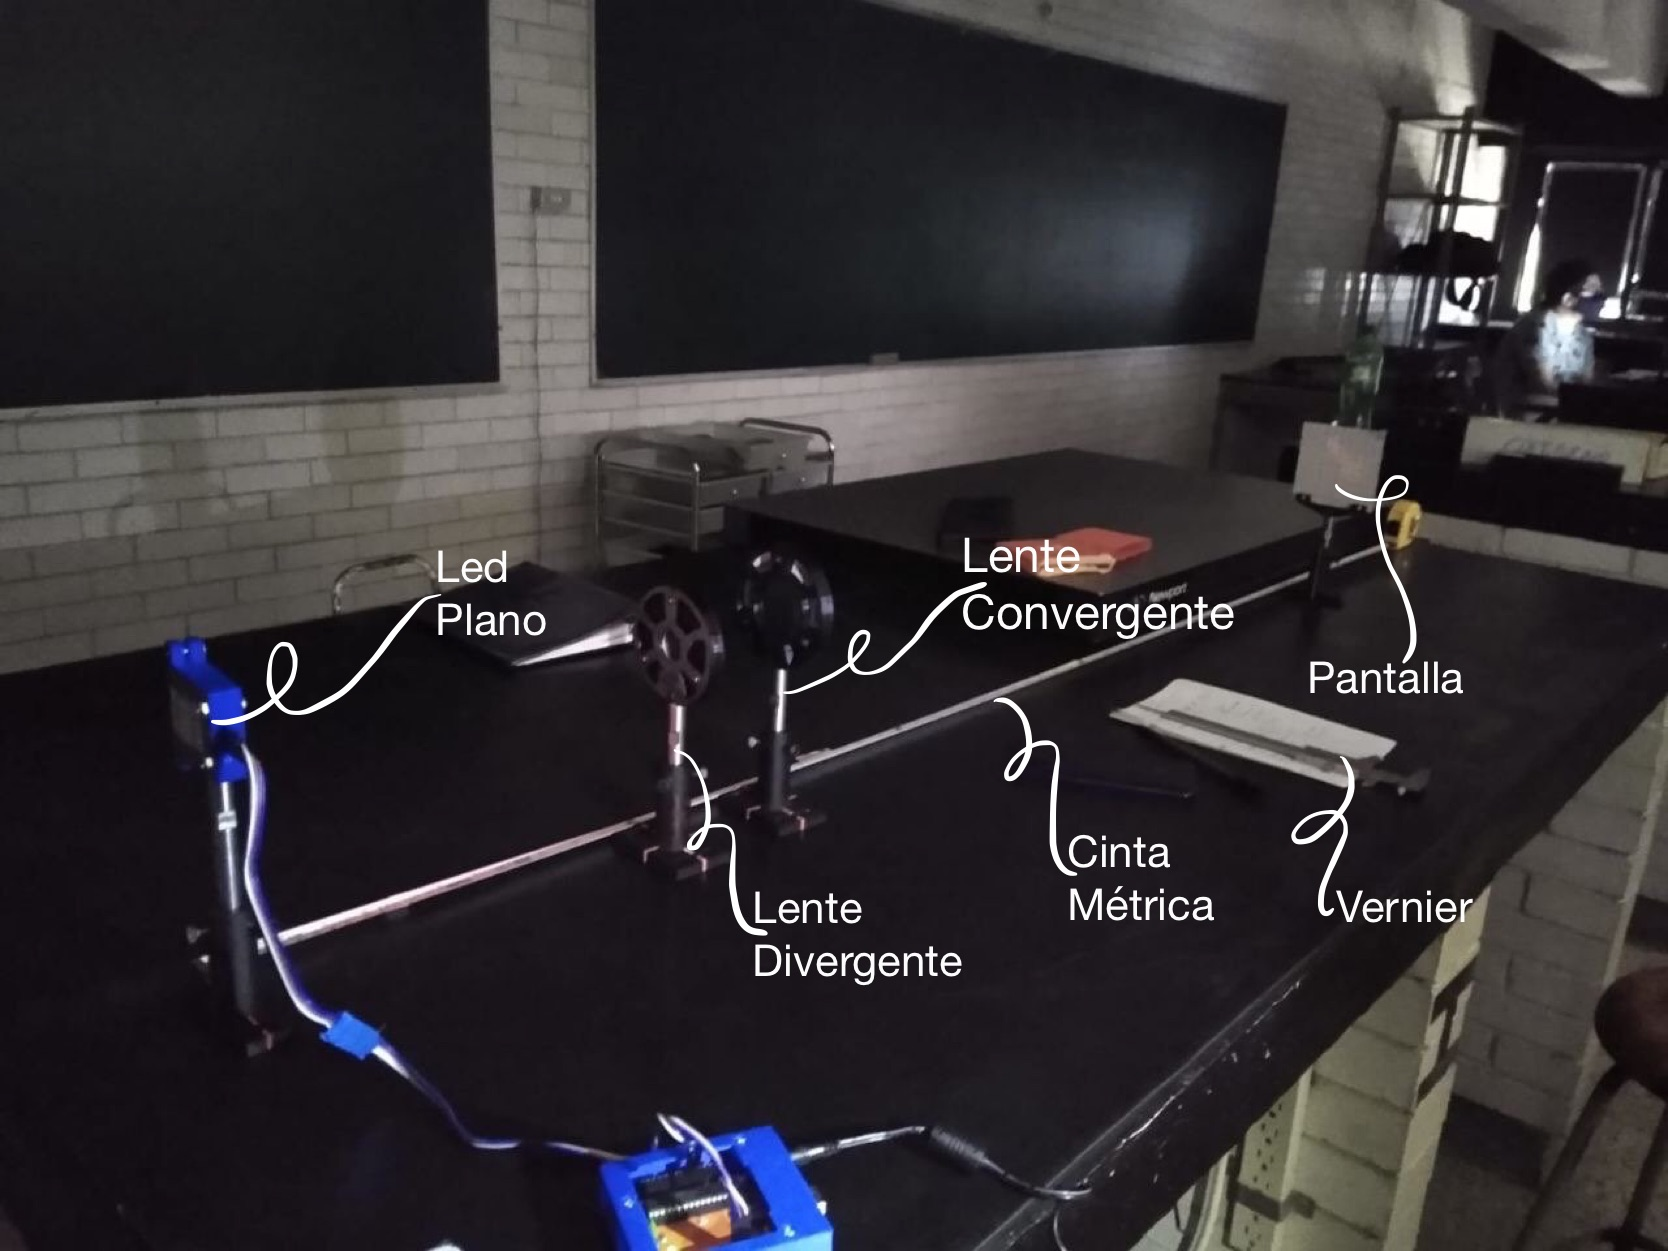
\includegraphics[width=0.25\textwidth]{imagenes/53A2B5A7-0059-4FA2-9216-A049663C24E5.jpeg}}
 \caption{En la figura 3(a) se muestra el arreglo experimental utilizado para comprobar el método de Bessel para lentes covergentes. En la figura 3(b) se muestra el arreglo experimental que se empleo para el método de Bessel para lentes divergentes.}
 \label{f:Desarrollo experimental}
\end{figure}
\subsection*{\textcolor{carmine}{Desplazamiento de imagen.}}
Sobre la mesa del laboratorio se colocó una cinta métrica pegada con cinta para que no se moviera y un LED plano con forma de flecha en la orilla donde estaba la posición cero frente a el se coloco una pantalla y entre ellas se la lente convergente y se buscó el punto donde la imagen se veía nítida.    Luego entre la lente convergente y la pantalla se colocó una lente divergente y la imagen se desenfocó por lo que se tuvo que ajustar la posición de la lente y de la pantalla hasta que de nuevo se viera la imagen cuando de obtuvo esto se midieron las posiciones a la que estaban y la imágenes proyectadas, el experimento se repitió para otra posición. nuevamente se detectó una incertidumbre $\sigma_{ap}=\pm\hspace{0.1cm}0.05\hspace{0.1cm}\text{ cm}$ para las posiciones y una $\sigma_{ap}=\pm\hspace{0.1cm}0.005\hspace{0.1cm}\text{ cm}$ para las medidas de las imágenes encontradas. 
\subsection*{\textcolor{carmine}{Índice de refracción de una lente.}}
Se colocó sobre la mesa óptica del laboratorio un esferómetro  se giró hasta que el tornillo tocara con la superficie de la mesa y se estableció que el cero se encontraba en $0.002\hspace{0.1cm}\text{cm}\pm0.001\hspace{0.1cm}\text{ cm}$, se identificó que el esferómetro tenía una incertidumbre de $\sigma_{ap}=0.001\hspace{0.1cm}\text{ cm}$. Luego se colocó sobre la lente convergente y se giró hasta tocar con la superficie del espejo, se contaron el número de vueltas. Con un vernier se midió la altura y se determinó que la incertidumbre estaba dada por $\sigma_{ap}=0.005\hspace{0.1cm}\text{ cm}$, el procedimiento se repitió 2 veces con los mismos instrumentos. 
\begin{figure}[H]
    \centering
    \subfloat[\textbf{Arreglo experimental.} Desplazamiento imagen]{
    \label{f:Arreglo experimental}
    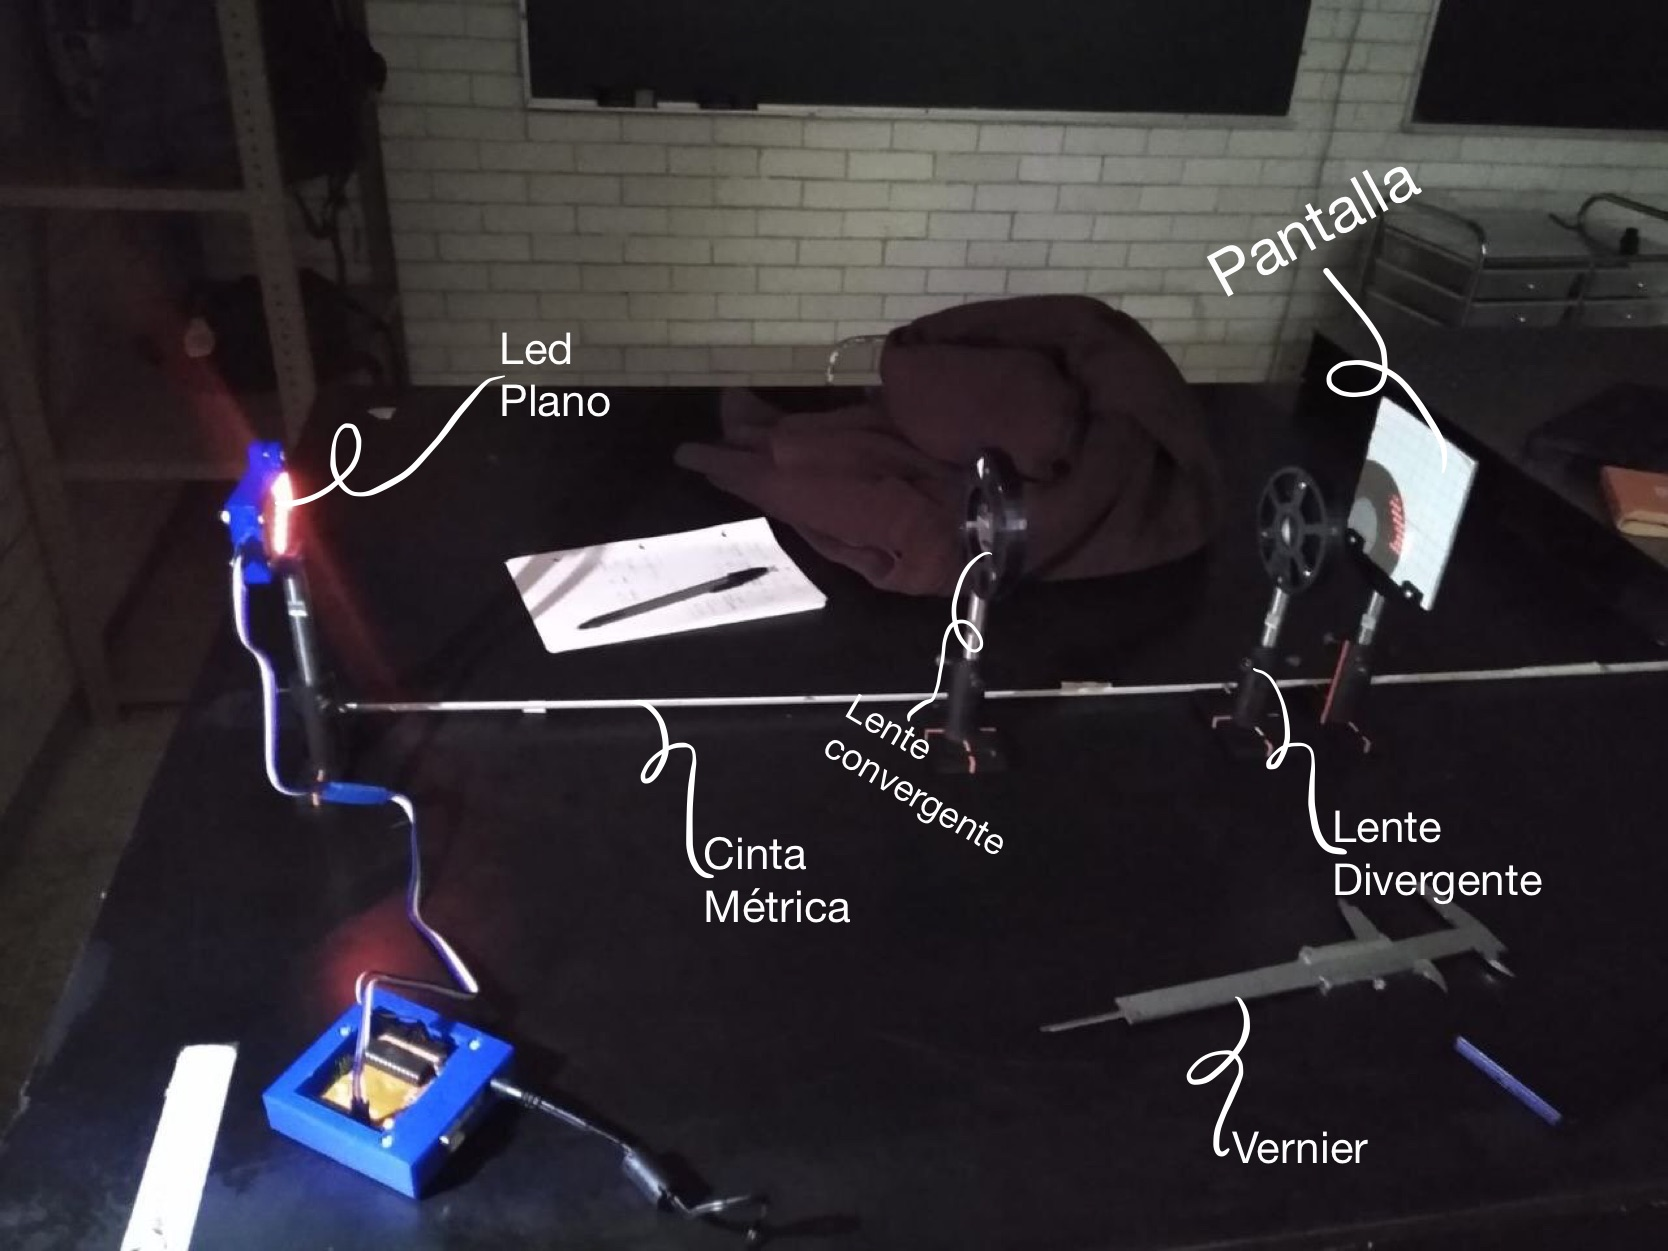
\includegraphics[width=5cm]{imagenes/BDA7617E-4874-488E-A964-40B2E174AB73.jpeg}}
    \subfloat[\textbf{Arreglo experimental.}Índice de Refracción]{
   \label{f:Lineas}
    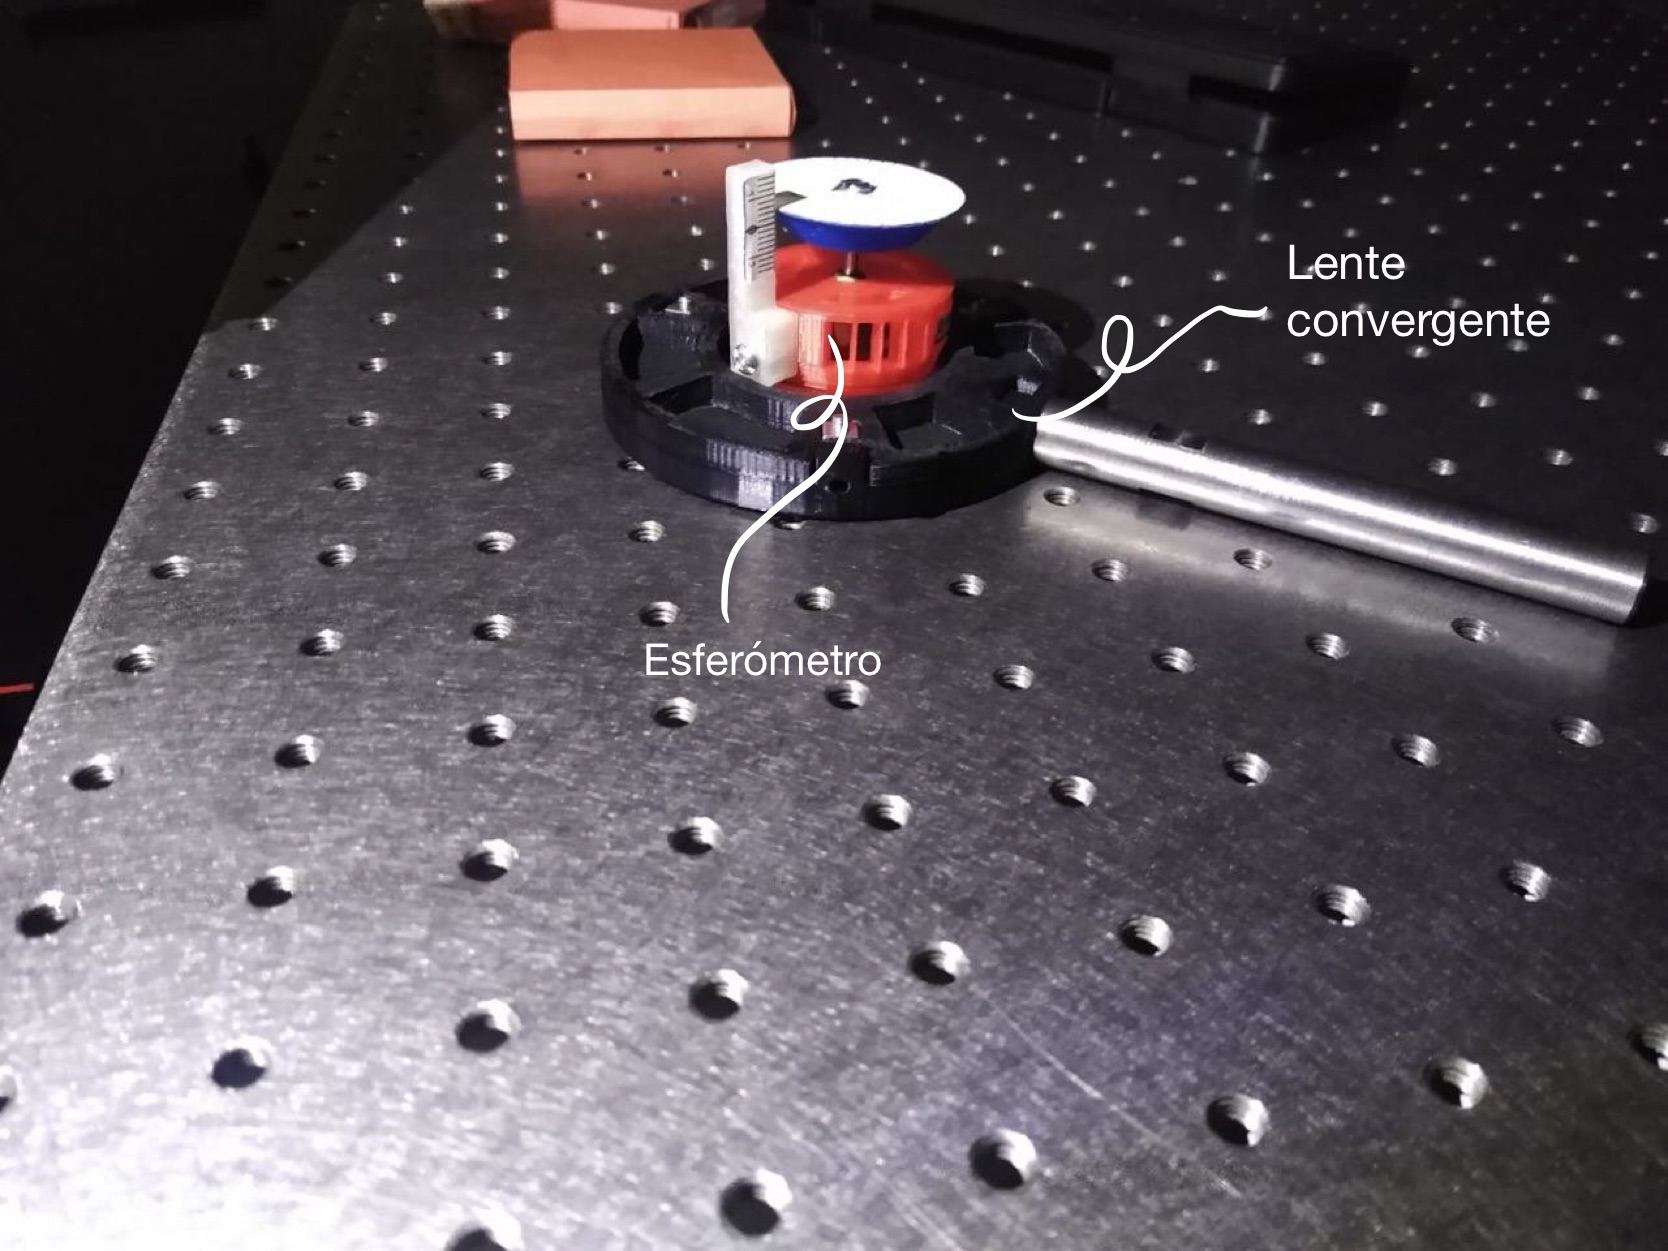
\includegraphics[width=0.25\textwidth]{imagenes/D6E517E1-C09B-4E41-B047-32F73431819B.jpeg}}
 \caption{Se observa el arreglo experimental 3(a) para el método de desplazamiento imagen con una lente divergente. En la figura 3(b) se observa el esferómetro sobre una lente convergente que es el arreglo experimental del método de índice de refracción de una lente..}
 \label{f:Desarrollo experimental}
\end{figure}
\section*{\textcolor{carmine}{Resultados y Análisis.}}


\subsection*{\textcolor{carmine}{Objeto al infinito.}}
La distancia entre la lente y la pantalla fue de:
\begin{equation*}
    i= (10.8 \pm 0.05) \text{ cm}
\end{equation*}
Por la ecuación $(2)$ y considerando la distancia entre el edificio y la lente como muy grande $\frac{1}{o}=\infty$, tenemos:
\begin{equation*}
    f_{\text{conv}}= (10.8 \pm 0.05) \text{ cm}
\end{equation*}



\subsection*{\textcolor{carmine}{Método gráfico.}}

Se linealizó la ecuación $(1)$ de la siguiente forma:

\begin{equation*}
    \frac{1}{o} =- \frac{1}{i} + \frac{1}{f}
\end{equation*}
\begin{figure}[H]
    \centering
    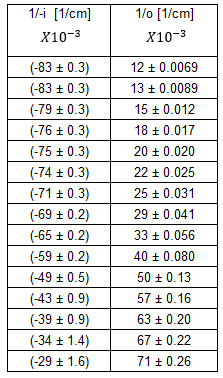
\includegraphics[scale=0.8]{tablas/tabla grafico.PNG}
    \caption{Tabla de distancias objeto e imagen.}
\end{figure}


\begin{figure}[H]
    \centering
    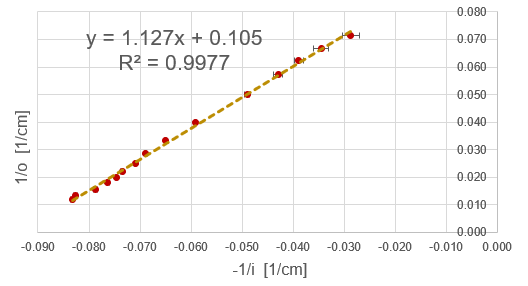
\includegraphics[scale=0.8]{graficass/metodo grafico.PNG}
    \caption{Gráfica de datos de la tabla en la figura 5 ajustados mínimos cuadrados.}
\end{figure}

De esta manera ajustando con el método de mínimos cuadrados se obtiene que la distancia focal con su respectiva incertidumbre es:

\begin{equation*}
    f = \frac{1}{b} \hspace{1cm} \Delta f = \frac{\Delta b}{b^2}
\end{equation*}

El ajuste da los siguientes valores:

\begin{equation*}
    f_{\text{conv}} = (9.493 \pm 0.087) \text{ cm}
\end{equation*}





\subsection*{\textcolor{carmine}{Bessel.}}

La distancia $b$ entre el objeto y la pantalla y la distancia entre las $2$ posiciones de la lente $a$ fue:

\begin{equation*}
    b= (58.2 \pm 0.1)  \text{ cm} \hspace{1cm} a = (31.8 \pm 0.1) \text{ cm}
\end{equation*}
Con estos datos se puede obtener la distancia focal mediante la ecuación $(4)$, donde se puede obtener la incertidumbre mediante la formula de propagación de errores:
\begin{equation*}
    \Delta f = \sqrt{\left(\frac{\partial f}{\partial b}\Delta b\right)^{2} + \left(\frac{\partial f}{\partial a} \Delta a\right)^{2}} = \sqrt{\left(\frac{b^2 - a^2}{4b}\Delta b\right)^{2} + \left(\frac{a^2}{2b}\Delta a\right)^{2}}
\end{equation*}
Esto da:
\begin{equation*}
    f_{\text{conv}} = (10.21 \pm 0.03) \text{ cm}
\end{equation*}




\subsection*{\textcolor{carmine}{Bessel para lentes divergentes.}}

\begin{equation*}
    f_{\text{conv}}= 10 \text{ cm} \hspace{1cm} a = (82.5 \pm 0.1) \text{ cm}
\end{equation*}

Despejando $b$ de la ecuación $(4)$ y propagando su incertidumbre:

\begin{equation*}
    b = \pm \sqrt{a^2 + 4f_{\text{conv}}^{2}} + 2f_{\text{conv}}
\end{equation*}

\begin{equation*}
    \Delta b = \left| \frac{\partial b}{\partial a}\Delta a\right|= \frac{a \Delta a}{2b}
\end{equation*}

La raíz positiva es:

\begin{equation*}
    b = (104.89 \pm 0.10) \text{ cm} 
\end{equation*}

\begin{equation*}
    i = (-7.11 \pm 0.20) \text{ cm} \hspace{1cm} o = (28 \pm 0.05) \text{ cm}
\end{equation*}

Despejando $f$ de la ecuación $(1)$ y propagando su incertidumbre:

\begin{equation*}
    f= \frac{1}{\frac{1}{o}+\frac{1}{i}}
\end{equation*}

\begin{equation*}
    \Delta f = \sqrt{\left(\frac{\partial f}{\partial o}\Delta o\right)^{2} + \left(\frac{\partial f}{\partial i}\Delta i\right)^{2}}
\end{equation*}


\begin{equation*}
    f_{\text{div}} =(-9.53 \pm 0.35 ) \text{ cm}
\end{equation*}

Despejando $h_i$ de la ecuación $(2)$ y propagando su incertidumbre:

\begin{equation*}
    h_i = h_o \frac{-i}{o}
\end{equation*}

\begin{equation*}
    \Delta h_i = \sqrt{\left(\frac{\partial h_i}{\partial h_o} \Delta h_o\right)^{2} + \left(\frac{\partial h_i}{\partial i}\Delta i\right)^{2} + \left(\frac{\partial h_i}{\partial o}\Delta o\right)^{2}}
\end{equation*}

\begin{figure}[H]
    \centering
    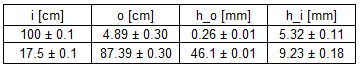
\includegraphics[scale=1]{tablas/tabla bessel.PNG}
    \caption{Tabla de distancias y tamaños objeto e imagen.}
\end{figure}

Promediando:

\begin{equation*}
    h_i = (7.27 \pm 0.15) \text{ mm}
\end{equation*}



\subsection*{\textcolor{carmine}{Desplazamiento de imagen.}}

Las distancias objeto e imagen son:

\begin{equation*}
    o = (-3.7 \pm 0.1) \text{ cm} \hspace{1cm} i = (6.1 \pm 0.1) \text{ cm}
\end{equation*}

Despejando $f$ de la ecuación $(1)$ y propagando su incertidumbre se obtiene:

\begin{equation*}
    f_{\text{div}} = (-9.40 \pm 0.69) \text{ cm}
\end{equation*}






\subsection*{\textcolor{carmine}{Índice de refracción de una lente.}}

Propagando la incertidumbre de la ecuación $(5)$:

\begin{equation*}
    \Delta R = \sqrt{\left(\frac{\partial R}{\partial a}\Delta a\right)^{2} + \left(\frac{\partial R}{\partial h} \Delta h\right)^{2}} =\frac{a}{2h} \sqrt{4\Delta a^2 + \Delta h^2 \left(\frac{a^2}{h^2} + \frac{h^2}{a^2}\right) }
\end{equation*}

Sabemos que:

\begin{equation*}
    f=\frac{R}{2}
\end{equation*}

Donde la incertidumbre esta dada por:

\begin{equation*}
    \Delta f = \frac{\Delta R}{2}
\end{equation*}

\begin{figure}[h!]
    \centering
    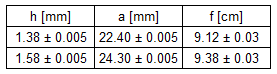
\includegraphics[scale=1]{tablas/esferometro.PNG}
    \caption{Tabla de focos calculados con el esferómetro.}
\end{figure}

Promediando focos y radios se obtiene:

\begin{equation*}
    R_1 = (18.5 \pm 0.6) \text{ cm} \hspace{1cm} R_2 = (-18.5 \pm 0.6) \text{ cm}
\end{equation*}

\begin{equation*}
    f_{\text{conv}}=(9.25 \pm 0.03) \text{ cm}
\end{equation*}

Despejando $n$ de la ecuación $(3)$ y propagando su incertidumbre se obtiene:

\begin{equation*}
    n= \frac{1}{f\left(\frac{1}{R_1} - \frac{1}{R_2}\right)} + 1 
\end{equation*}

\begin{equation*}
    \Delta n = \sqrt{\left(\frac{\partial n}{\partial f} \Delta f\right)^{2} + \left(\frac{\partial n}{\partial R_1}  \Delta R_1\right)^{2} + \left(\frac{\partial n}{\partial R_2} \Delta R_2\right)^{2}}
\end{equation*}

\begin{equation*}
    = \frac{1}{f^2\left(\frac{1}{R_1} - \frac{1}{R_2}\right)^{2}} \sqrt{\left(\Delta f (\frac{1}{R_1}- \frac{1}{R_2})\right)^{2}+\left(\frac{\Delta R_1 f}{R_{1}^{2}}\right)^{2} + \left(\frac{\Delta R_2 f}{R_{2}^{2}}\right)^{2}}
\end{equation*}

Sustituyendo los datos y simplificando tenemos:

\begin{equation*}
    n = (2 \pm 0.2)
\end{equation*}

\section*{\textcolor{carmine}{Discusión y Conclusión.}}
Debido a que el edificio no estaba lo suficiente alejado entonces solo se obtuvo una aproximación, con el método Objeto al infinito, para la distancia focal, esta aproximación fue:
$$ f_{\text{conv}}=(10.8\pm 0.05)\text{ cm} $$
Para el método gráfico se obtuvo:
$$ f_{\text{conv}}=(9.493\pm 0.087)\text{ cm} $$
Mientras que con el método de Bessel:
$$ f_{\text{conv}}=(10.21\pm 0.03)\text{ cm}  $$
Podemos ver que los resultados de la distancia focal de la lente convergente oscilan respecto al valor de fabrica $f=10\text{ cm}$, algunos resultados nos dieron un valor menor y otros un valor mayor. Cada método se acercó al valor esperado pero al final no fueron exactos, esto puede corregirse tomando con mayor precaución los datos.
\\\\
Usando el metodo de Bessel para lentes divergentes se obtuve que la distancia focal de la lente divergente es:
$$ f_{\text{div}}=(-9.53\pm 0.35)\text{ cm} $$
Mientras que el tamaño de la imagen virtual que estaba frente a la lente divergente fue:
$$ h_{i}=(7.27\pm0.15)mm $$
Con el metodo de desplazamiento de imagen se obtuvo que la longitud focal de la lente divergente es:
$$ f_{\text{div}}=(-9.40\pm 0.69)\text{ cm} $$
Con el esferómetro se obtuvo que la longitud focal de la lente convergente es:
$$ f_{\text{conv}}=(9.25\pm 0.03)\text{ cm} $$
Y se encontró que el índice de refracción del material del que están hechas las lentes es:
$$ n=(2\pm0.2) $$
%$n=1.514$
\nocite{*}

\bibliography{biblio}
\subsection*{\textcolor{carmine}{Apéndice}}
Ecuación del esferómetro
\begin{equation}
    R= \frac{a^2}{2h}+\frac{h}{2}
\end{equation}
\end{document}